\documentclass{article}
\usepackage[utf8]{inputenc}
\usepackage{polski}
\usepackage{tikz}
\usepackage[margin=2cm]{geometry} %margins
\usetikzlibrary{shadows.blur} %imports shadows function from tkzlibrary
\pagestyle{empty} %no headers footers no page number 
\usetikzlibrary{arrows.meta}


\tikzset{
    mynode/.style={font=\rmfamily\mdseries\normalsize}
}

\begin{document}
    \begin{center}
    
        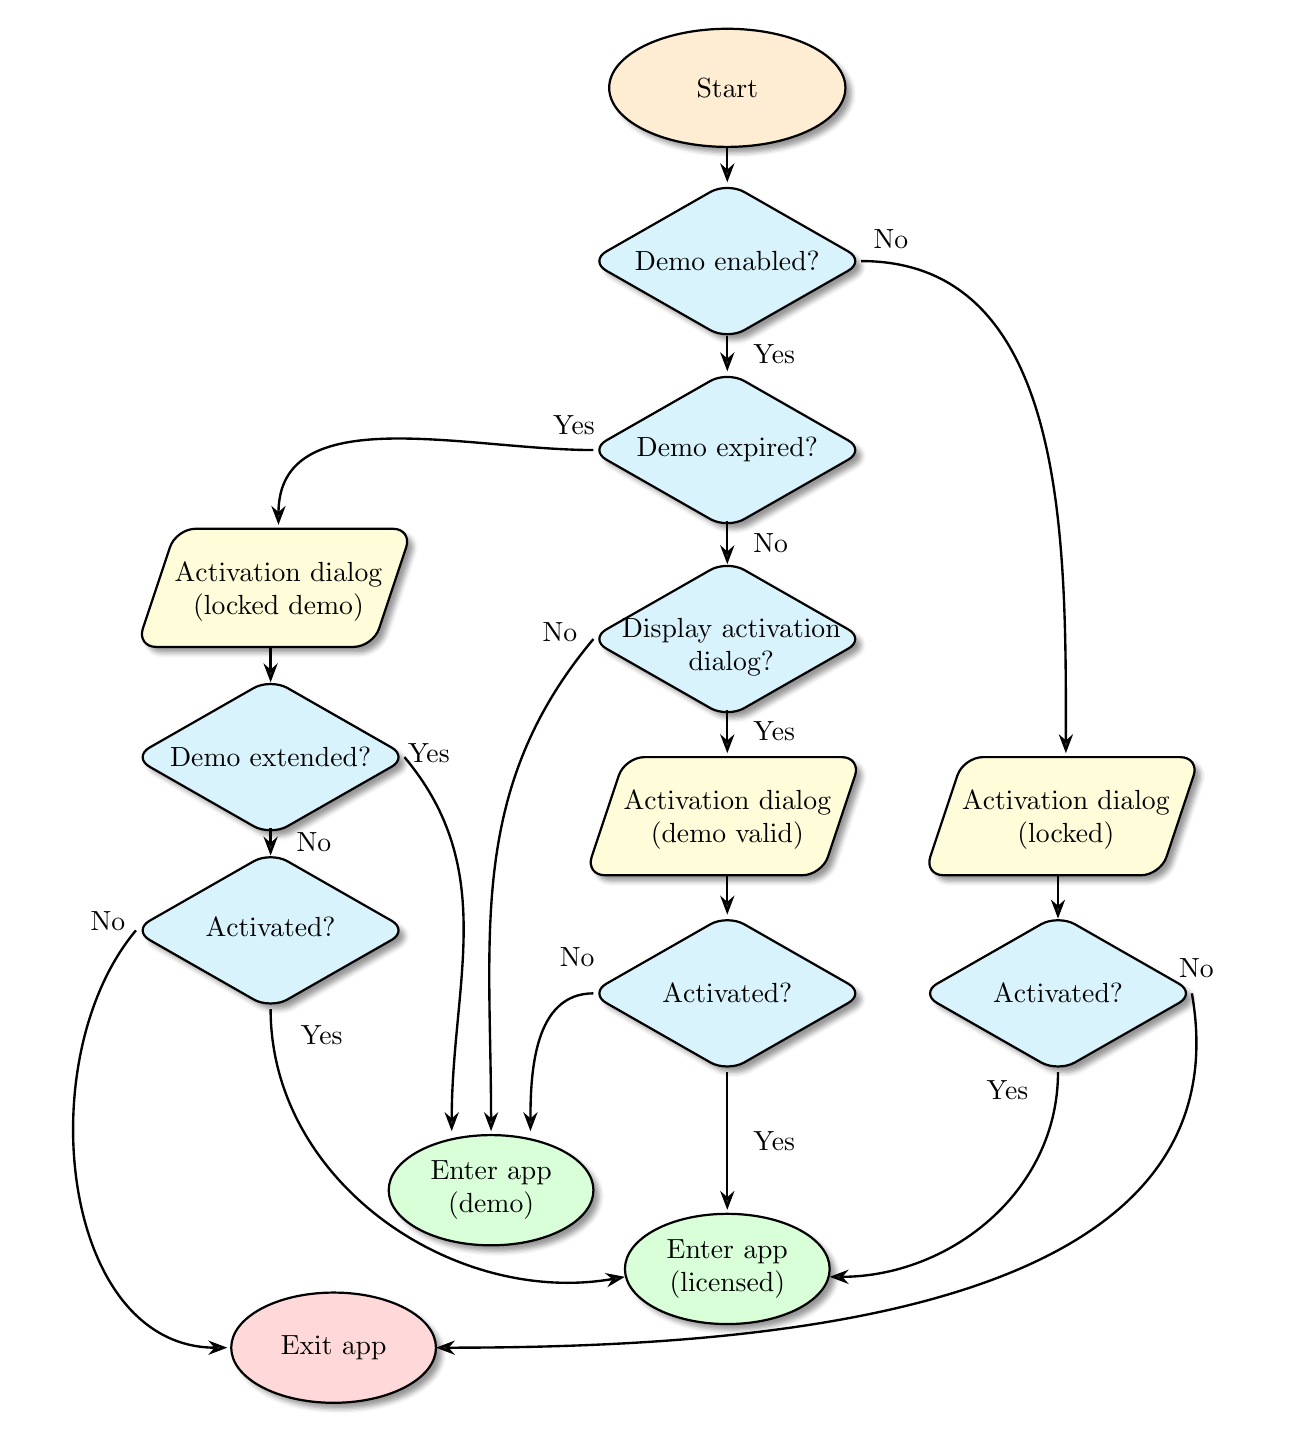
\begin{tikzpicture}
        % figures 
        \filldraw[fill=yellow!15!orange!15,thick,blur shadow] (0,0) ellipse (1.5 and  0.75);
        \node[mynode,align=center,thin] at (0,0) {Start}; % elipse
        
         \filldraw[fill=cyan!15,thick,rounded corners=7,blur shadow] (0,-1.2) -- ++(1.75,-1) -- ++(-1.75,-1) -- ++(-1.75,1) -- cycle;
        \node[mynode,align=center,thin] at (0,-2.2) {Demo enabled?};% rhombus
        
        \filldraw[fill=cyan!15,thick,rounded corners=7,blur shadow] (0,-3.6) -- ++(1.75,-1) -- ++(-1.75,-1) -- ++(-1.75,1) -- cycle;
        \node[mynode,align=center,thin] at (0,-4.6) {Demo expired?};% rhombus

        \filldraw[fill=cyan!15,thick,rounded corners=7,blur shadow] (0,-6) -- ++(1.75,-1) -- ++(-1.75,-1) -- ++(-1.75,1) -- cycle;
        \node[mynode,align=center,thin] at (0.05,-7.1) {Display activation\\dialog?};% rhombus

         \filldraw[fill=yellow!15,thick,rounded corners=7,blur shadow] (-4,-5.6) -- ++(-3,0) -- ++(-0.5,-1.5) -- ++(3,0) -- cycle;
        \node[mynode,align=center,thin] at (-5.7,-6.4) {Activation dialog \\(locked demo)}; %parallelogram

        \filldraw[fill=yellow!15,thick,rounded corners=7,blur shadow] (1.7,-8.5) -- ++(-3,0) -- ++(-0.5,-1.5) -- ++(3,0) -- cycle;
        \node[mynode,align=center,thin] at (0,-9.3) {Activation dialog \\(demo valid)};
        %parallelogram
        
        \filldraw[fill=yellow!15,thick,rounded corners=7,blur shadow] (6,-8.5) -- ++(-3,0) -- ++(-0.5,-1.5) -- ++(3,0) -- cycle;
        \node[mynode,align=center,thin] at (4.3,-9.3) {Activation dialog \\(locked)};
        %parallelogram

        \filldraw[fill=cyan!15,thick,rounded corners=7,blur shadow] (0,-10.5) -- ++(1.75,-1) -- ++(-1.75,-1) -- ++(-1.75,1) -- cycle;
        \node[mynode,align=center,thin] at (0,-11.5) {Activated?};% rhombus

        \filldraw[fill=cyan!15,thick,rounded corners=7,blur shadow] (4.2,-10.5) -- ++(1.75,-1) -- ++(-1.75,-1) -- ++(-1.75,1) -- cycle;
        \node[mynode,align=center,thin] at (4.2,-11.5) {Activated?};% rhombus

        \filldraw[fill=cyan!15,thick,rounded corners=7,blur shadow] (-5.8,-7.5) -- ++(1.75,-1) -- ++(-1.75,-1) -- ++(-1.75,1) -- cycle;
        \node[mynode,align=center,thin] at (-5.8,-8.5) {Demo extended?};% rhombus

        \filldraw[fill=cyan!15,thick,rounded corners=7,blur shadow] (-5.8,-9.7) -- ++(1.75,-1) -- ++(-1.75,-1) -- ++(-1.75,1) -- cycle;
        \node[mynode,align=center,thin] at (-5.8,-10.65) {Activated?};% rhombus

        \filldraw[fill=green!15,thick,blur shadow] (-3,-14) ellipse (1.3 and  0.7);
        \node[mynode,align=center,thin] at (-3,-14) {Enter app \\(demo)}; % elipse

        \filldraw[fill=green!15,thick,blur shadow] (0,-15) ellipse (1.3 and  0.7);
        \node[mynode,align=center,thin] at (0,-15) {Enter app \\(licensed)}; % elipse

        \filldraw[fill=red!15,thick,blur shadow] (-5,-16) ellipse (1.3 and  0.7);
        \node[mynode,align=center,thin] at (-5,-16) {Exit app}; % elipse

        %arrows
        \draw [-{Stealth[scale=1]}, line width=0.3mm]  (0,-0.75) -- (0,-1.2);
        \draw [-{Stealth[scale=1]}, line width=0.3mm]   (0,-3.15) -- node[mynode,right,inner sep=9] {Yes} (0,-3.6) ;
        \draw [-{Stealth[scale=1]}, line width=0.3mm]   (1.7,-2.2) to [out=0,in=90] node[mynode,pos=0.05,above,inner sep=5] {No} (4.3,-8.45) ;
        \draw [-{Stealth[scale=1]}, line width=0.3mm]   (-5.8,-7.1) -- (-5.8,-7.55) ;
        \draw [-{Stealth[scale=1]}, line width=0.3mm]   (-5.8,-9.4) -- node[mynode,pos=0.5,right,inner sep=9] {No} (-5.8,-9.75) ;
        \draw [-{Stealth[scale=1]}, line width=0.3mm]   (-4.1,-8.5) to [out=-50,in=90] node[mynode,pos=0.10,above,inner sep=10] {Yes} (-3.5,-13.25) ;
        \draw [-{Stealth[scale=1]}, line width=0.3mm]   (-1.7,-7) to [out=230,in=90] node[mynode,pos=0.10,above,inner sep=15] {No} (-3,-13.25) ;
        \draw [-{Stealth[scale=1]}, line width=0.3mm]   (-1.7,-11.5) to [out=180,in=90] node[mynode,pos=0.10,above,inner sep=10] {No} (-2.5,-13.25) ;
        \draw [-{Stealth[scale=1]}, line width=0.3mm]   (4.2,-10) -- (4.2,-10.55) ;        
        \draw [-{Stealth[scale=1]}, line width=0.3mm]   (-5.8,-11.7) to [out=270,in=190] node[mynode,pos=0.05,right,inner sep=10] {Yes} (-1.3,-15.1) ;
        \draw [-{Stealth[scale=1]}, line width=0.3mm]   (-7.51,-10.7) to [out=230,in=180] node[mynode,pos=0.10,above,inner sep=15] {No} (-6.35,-16) ; 
        \draw [-{Stealth[scale=1]}, line width=0.3mm ]   (-1.7,-4.6) to [out=180,in=90] node[mynode,pos=0.05,above,inner sep=5] {Yes} (-5.7,-5.55) ;
        \draw [-{Stealth[scale=1]}, line width=0.3mm]   (0,-5.5) -- node[mynode,pos=0.5,right,inner sep=9] {No} (0,-6.05) ;
        \draw [-{Stealth[scale=1]}, line width=0.3mm]   (0,-7.9) -- node[mynode,pos=0.5,right,inner sep=9] {Yes} (0,-8.45) ;
        \draw [-{Stealth[scale=1]}, line width=0.3mm]   (0,-10) --   (0,-10.5) ;
        \draw [-{Stealth[scale=1]}, line width=0.3mm]   (0,-12.5) -- node[mynode,pos=0.5,right,inner sep=9] {Yes} (0,-14.25) ;
        \draw [-{Stealth[scale=1]}, line width=0.3mm]   (4.2,-12.5) to [out=270,in=0] node[mynode,pos=0.05,left,inner sep=10] {Yes} (1.3,-15.1) ; 
        \draw [-{Stealth[scale=1]}, line width=0.3mm]   (5.9,-11.5) to [out=280,in=0] node[mynode,pos=0.05,above,inner sep=22] {No} (-3.7,-16) ;



        
        
        
        
        \end{tikzpicture}
    \end{center}
\end{document}
   